\let\negmedspace\undefined
\let\negthickspace\undefined
\def\inputGnumericTable{}  
\documentclass[journal,12pt,onecolumn]{IEEEtran}
\usepackage{cite}
\usepackage{amsmath,amssymb,amsfonts,amsthm}
\usepackage{algorithmic}
\usepackage{graphicx}
\usepackage{textcomp}
\usepackage{xcolor}
\usepackage{txfonts}
\usepackage{listings}
\usepackage{enumitem}
\usepackage{mathtools}
\usepackage{gensymb}
\usepackage[breaklinks=true]{hyperref}
\usepackage{tkz-euclide} % loads  TikZ and tkz-base
\usepackage{listings}
\usepackage{gvv}
\usepackage[latin1]{inputenc}                                 
\usepackage{color}                                            
\usepackage{array}                                            
\usepackage{longtable}                                        
\usepackage{calc}                                             
\usepackage{multirow}                                         
\usepackage{hhline}                                           
\usepackage{ifthen}                                           
\usepackage{lscape}
\usepackage{bm}  
%
%\usepackage{setspace}
%\usepackage{gensymb}
%\doublespacing
%\singlespacing

%\usepackage{graphicx}
%\usepackage{amssymb}
%\usepackage{relsize}
%\usepackage[cmex10]{amsmath}
%\usepackage{amsthm}
%\interdisplaylinepenalty=2500
%\savesymbol{iint}
%\usepackage{txfonts}
%\restoresymbol{TXF}{iint}
%\usepackage{wasysym}
%\usepackage{amsthm}
%\usepackage{iithtlc}
%\usepackage{mathrsfs}
%\usepackage{txfonts}
%\usepackage{stfloats}
%\usepackage{bm}
%\usepackage{cite}
%\usepackage{cases}
%\usepackage{subfig}
%\usepackage{xtab}
%\usepackage{longtable}
%\usepackage{multirow}
%\usepackage{algorithm}
%\usepackage{algpseudocode}
%\usepackage{enumitem}
%\usepackage{mathtools}
%\usepackage{tikz}
%\usepackage{circuitikz}
%\usepackage{verbatim}
%\usepackage{tfrupee}
%\usepackage{stmaryrd}
%\usetkzobj{all}
%    \usepackage{color}                                            %%
%    \usepackage{array}                                            %%
%    \usepackage{longtable}                                        %%
%    \usepackage{calc}                                             %%
%    \usepackage{multirow}                                         %%
%    \usepackage{hhline}                                           %%
%    \usepackage{ifthen}                                           %%
  %optionally (for landscape tables embedded in another document): %%
%    \usepackage{lscape}     
%\usepackage{multicol}
%\usepackage{chngcntr}
%\usepackage{enumerate}

%\usepackage{wasysym}
%\documentclass[conference]{IEEEtran}
%\IEEEoverridecommandlockouts
% The preceding line is only needed to identify funding in the first footnote. If that is unneeded, please comment it out.

\newtheorem{theorem}{Theorem}[section]
\newtheorem{problem}{Problem}
\newtheorem{proposition}{Proposition}[section]
\newtheorem{lemma}{Lemma}[section]
\newtheorem{corollary}[theorem]{Corollary}
\newtheorem{example}{Example}[section]
\newtheorem{definition}[problem]{Definition}
%\newtheorem{thm}{Theorem}[section] 
%\newtheorem{defn}[thm]{Definition}
%\newtheorem{algorithm}{Algorithm}[section]
%\newtheorem{cor}{Corollary}
\newcommand{\BEQA}{\begin{eqnarray}}
\newcommand{\EEQA}{\end{eqnarray}}
\newcommand{\define}{\stackrel{\triangle}{=}}
\theoremstyle{remark}
\newtheorem{rem}{Remark}

%\bibliographystyle{ieeetr}
\begin{document}
%

\bibliographystyle{IEEEtran}


\vspace{3cm}

\title{
%	\logo{
Assignment
%	}
}
\author{ Aryan Jain - EE22BTECH11011$^{*}$% <-this % stops a space	
}	
%\title{
%	\logo{Matrix Analysis through Octave}{\begin{center}\includegraphics[scale=.24]{tlc}\end{center}}{}{HAMDSP}
%}


% paper title
% can use linebreaks \\ within to get better formatting as desired
%\title{Matrix Analysis through Octave}
%
%
% author names and IEEE memberships
% note positions of commas and nonbreaking spaces ( ~ ) LaTeX will not break
% a structure at a ~ so this keeps an author's name from being broken across
% two lines.
% use \thanks{} to gain access to the first footnote area
% a separate \thanks must be used for each paragraph as LaTeX2e's \thanks
% was not built to handle multiple paragraphs
%

%\author{<-this % stops a space
%\thanks{}}
%}
% note the % following the last \IEEEmembership and also \thanks - 
% these prevent an unwanted space from occurring between the last author name
% and the end of the author line. i.e., if you had this:
% 
% \author{....lastname \thanks{...} \thanks{...} }
%                     ^------------^------------^----Do not want these spaces!
%
% a space would be appended to the last name and could cause every name on that
% line to be shifted left slightly. This is one of those "LaTeX things". For
% instance, "\textbf{A} \textbf{B}" will typeset as "A B" not "AB". To get
% "AB" then you have to do: "\textbf{A}\textbf{B}"
% \thanks is no different in this regard, so shield the last } of each \thanks
% that ends a line with a % and do not let a space in before the next \thanks.
% Spaces after \IEEEmembership other than the last one are OK (and needed) as
% you are supposed to have spaces between the names. For what it is worth,
% this is a minor point as most people would not even notice if the said evil
% space somehow managed to creep in.



% The paper headers
%\markboth{Journal of \LaTeX\ Class Files,~Vol.~6, No.~1, January~2007}%
%{Shell \MakeLowercase{\textit{et al.}}: Bare Demo of IEEEtran.cls for Journals}
% The only time the second header will appear is for the odd numbered pages
% after the title page when using the twoside option.
% 
% *** Note that you probably will NOT want to include the author's ***
% *** name in the headers of peer review papers.                   ***
% You can use \ifCLASSOPTIONpeerreview for conditional compilation here if
% you desire.




% If you want to put a publisher's ID mark on the page you can do it like
% this:
%\IEEEpubid{0000--0000/00\$00.00~\copyright~2007 IEEE}
% Remember, if you use this you must call \IEEEpubidadjcol in the second
% column for its text to clear the IEEEpubid mark.



% make the title area
\maketitle



%\tableofcontents

\bigskip

\renewcommand{\thefigure}{\theenumi}
\renewcommand{\thetable}{\theenumi}
%\renewcommand{\theequation}{\theenumi}

%\begin{abstract}
%%\boldmath
%In this letter, an algorithm for evaluating the exact analytical bit error rate  (BER)  for the piecewise linear (PL) combiner for  multiple relays is presented. Previous results were available only for upto three relays. The algorithm is unique in the sense that  the actual mathematical expressions, that are prohibitively large, need not be explicitly obtained. The diversity gain due to multiple relays is shown through plots of the analytical BER, well supported by simulations. 
%
%\end{abstract}
% IEEEtran.cls defaults to using nonbold math in the Abstract.
% This preserves the distinction between vectors and scalars. However,
% if the journal you are submitting to favors bold math in the abstract,
% then you can use LaTeX's standard command \boldmath at the very start
% of the abstract to achieve this. Many IEEE journals frown on math
% in the abstract anyway.

% Note that keywords are not normally used for peerreview papers.
%\begin{IEEEkeywords}
%Cooperative diversity, decode and forward, piecewise linear
%\end{IEEEkeywords}



% For peer review papers, you can put extra information on the cover
% page as needed:
% \ifCLASSOPTIONpeerreview
% \begin{center} \bfseries EDICS Category: 3-BBND \end{center}
% \fi
%
% For peerreview papers, this IEEEtran command inserts a page break and
% creates the second title. It will be ignored for other modes.
%\IEEEpeerreviewmaketitle
\textbf{Question}:
Suppose that $\vec{X_1}, \vec{X_2},\ldots, \vec{X_n}, \vec{Y_1}, \vec{Y_2},\ldots, \vec{Y_n}$ are independent and identically distributed random vectors each having $N_p\brak{\bm{\mu},\Sigma}$ distributions, where $\Sigma$ is non-singular, $p>1$ and $n>1$. If $\vec{X} = \frac{1}{n}\sum_{i=1}^{n}\vec{X_i}$ and $\vec{Y} = \frac{1}{n}\sum_{i=1}^{n}\vec{Y_i}$, then which one of the following statements is true?
\begin{enumerate}[label=(\alph*)]
\item There exists $c>0$ such that $c{\brak{\vec{X}-\bm{\mu}}}^T{\Sigma}^{-1}\brak{\vec{X}-\bm{\mu}}$ has ${\chi}^2$-distribution with $p$ degrees of freedom.
\item There exists $c>0$ such that $c{\brak{\vec{X}-\vec{Y}}^T}{\Sigma}^{-1}\brak{\vec{X}-\vec{Y}}$ has ${\chi}^2$-distribution with $\brak{p-1}$ degrees of freedom.
\item There exists $c>0$ such that $c\sum_{i=1}^n{\brak{\vec{X_i}-\vec{X}}}^T{\Sigma}^{-1}\brak{\vec{X_i}-\vec{X}}$ has ${\chi}^2$-distribution with $p$ degrees of freedom.
\item There exists $c>0$ such that $c\sum_{i=1}^n{\brak{\vec{X_i}-\vec{Y_i}-\vec{X}+\vec{Y}}}^T{\Sigma}^{-1}\brak{\vec{X_i}-\vec{Y_i}-\vec{X}+\vec{Y}}$ has ${\chi}^2$-distribution with $p$ degrees of freedom.   \hfill{GATE ST Paper 2023} 
\end{enumerate}    
\solution
\newline
We are given that,
\begin{align}
\vec{X_1}, \vec{X_2},\ldots, \vec{X_n}, \vec{Y_1}, \vec{Y_2},\ldots, \vec{Y_n} \sim N_p\brak{\bm{\mu},\Sigma}
\end{align}
Also,
\begin{align}
\vec{X} &= \frac{1}{n}\sum_{i=1}^{n}\vec{X_i} \\
\vec{Y} &= \frac{1}{n}\sum_{i=1}^{n}\vec{Y_i} 
\end{align}
The mean of $\vec{X}$ is given by: 
\begin{align}
{\bm{\mu}}_{\vec{X}} &= E\brak{\vec{X}} \\
                                    &= \frac{1}{n}\sum_{i=1}^{n}E\brak{\vec{X_i}} \\
                                    &= \bm{\mu}  \label{eq:23/25/1}
\end{align}
Similarly,
\begin{align}
{\bm{\mu}}_{\vec{Y}} &= \bm{\mu}
\end{align}
The covariance of $\vec{X}$ is given by: 
\begin{align}
\Sigma_{\vec{X}} &= E\sbrak{\brak{\vec{X}-\bm{\mu}}{\brak{\vec{X}-\bm{\mu}}}^T} \\
                 &= E\sbrak{\brak{\frac{1}{n}\sum_{i=1}^{n}\vec{X_i}-\bm{\mu}}{\brak{\frac{1}{n}\sum_{i=1}^{n}\vec{X_i}-\bm{\mu}}}^T} \\
                 &= \frac{1}{n^2}E\sbrak{\sum_{i=1}^{n}\brak{\vec{X_i}-\bm{\mu}}{\brak{\vec{X_i}-\bm{\mu}}}^T} \\
                 &= \frac{1}{n^2}\sbrak{\sum_{i=1}^{n}E\brak{{\vec{X_i}}^2+{\bm{\mu}}^2-2\bm{\mu}\vec{X_i}}} \\
                 &= \frac{1}{n^2}\sbrak{\sum_{i=1}^{n}E\brak{{\vec{X_i}}^2}+\sum_{i=1}^{n}E\brak{{\bm{\mu}}^2}-2\bm{\mu}\sum_{i=1}^{n}E\brak{\vec{X_i}}} \\
                 &= \frac{1}{n^2}\sbrak{n\Sigma+n{\bm{\mu}}^2+n{\bm{\mu}}^2-2{\bm{\mu}}^2} \quad \sbrak{\because E\brak{{\vec{X_i}}^2}={\Sigma}_{\vec{X_i}}+{E\brak{\vec{X_i}}}^2} \\
                 &= \frac{\Sigma}{n}         
\end{align}
Similarly,
\begin{align}
\Sigma_{\vec{Y}} &= \frac{\Sigma}{n} 
\end{align}
\begin{enumerate}[label=(\alph*)]
\item To check option (A): \\
let us say,
\begin{align}
\vec{A} &= c{\brak{\vec{X}-\bm{\mu}}}^T{\Sigma}^{-1}\brak{\vec{X}-\bm{\mu}} \\
\end{align}
And,
\begin{align}
{\Sigma}^{-1} &= {\vec{F}}^T\vec{F} \label{eq:23/25/3} \\
\vec{y} &= \vec{F}\brak{\vec{X}-\bm{\mu}} \\
\implies \vec{A} &= c{\vec{y}}^T\overline{\vec{y}} \\
                 &= c{\norm{\vec{y}}}^2  \label{eq:23/25/2}
\end{align}
Equation \eqref{eq:23/25/2} shows that $\vec{A}$ can have ${\chi}^2$-distribution. \\
To confirm that we will find the mean and covariance-matrix of $\overline{\vec{y}}$.
\begin{align}
{\bm{\mu}}_{\vec{y}} &= E\brak{\vec{y}} \\
                           &= E\brak{\vec{F}\brak{\vec{X}-\bm{\mu}}} \\
                           &= \vec{F}\sbrak{E\brak{\vec{X}}-E\brak{\bm{\mu}}} \\
                           &= \vec{F}\sbrak{\bm{\mu}-\bm{\mu}} \quad from \eqref{eq:23/25/1} \\
                           &= 0 
\end{align}
And,
\begin{align}
{\Sigma}_{\vec{y}} &= E\sbrak{\brak{\vec{y}-{\bm{\mu}}_{\vec{y}}}{\brak{\vec{y}-{\bm{\mu}}_{\vec{y}}}}^T} \\
                              &= E\sbrak{\brak{\vec{F}\brak{\vec{X}-\bm{\mu}}}{\brak{\vec{F}\brak{\vec{X}-\bm{\mu}}}}^T} \\
                              &= E\sbrak{\vec{F}\brak{\vec{X}-\bm{\mu}}{\brak{\vec{X}-\bm{\mu}}}^T{\vec{F}}^T} \\
                              &= \vec{F}\sbrak{E\sbrak{\brak{\vec{X}-\bm{\mu}}{\brak{\vec{X}-\bm{\mu}}}^T}}{\vec{F}}^T \\
                              &= \vec{F} \Sigma {\vec{F}}^T 
\end{align}
since,
\begin{align}
{\Sigma}^{-1} &= {\vec{F}}^T\vec{F} \\
\Sigma{\Sigma}^{-1} &= \Sigma{\vec{F}}^T\vec{F} \\
\vec{I} &= \Sigma{\vec{F}}^T\vec{F} \\
\vec{I}{\vec{F}}^{-1} &= \Sigma{\vec{F}}^T \\
\vec{F}{\vec{F}}^{-1} &= \vec{F}\Sigma{\vec{F}}^T \\
\vec{I} &= \vec{F}\Sigma{\vec{F}}^T    \label{eq:23/25/4}
\end{align}
So using \eqref{eq:23/25/4},
\begin{align}
{\Sigma}_{\vec{y}} &= \vec{I}
\end{align}
Hence, For $c=1$ $\vec{A}$ has ${\chi}^2$-distribution with p degrees of freedom. \\
So option (A) is correct. 
\begin{figure}[!ht]
\centering
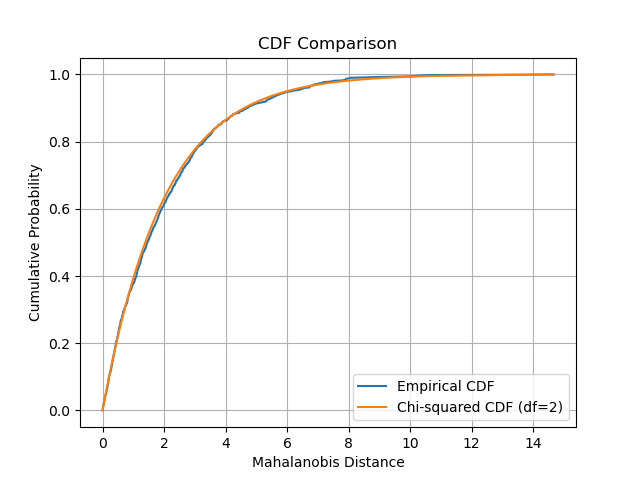
\includegraphics[width=\columnwidth]{./figs/graph.png}
\end{figure}
\item To check option (B): \\
Let us say,
\begin{align}
\vec{B} &= c{\brak{\vec{X}-\vec{Y}}^T}{\Sigma}^{-1}\brak{\vec{X}-\vec{Y}}
\end{align}
And,
\begin{align}
{\Sigma}^{-1} &= {\vec{F}}^T\vec{F}  \\
\vec{y} &= \vec{F}\brak{\vec{X}-\vec{Y}} \\
\implies \vec{B} &= c{\vec{y}}^T\overline{\vec{y}} \\
                 &= c{\norm{\vec{y}}}^2  \label{eq:23/25/5}
\end{align}
Equation \eqref{eq:23/25/5} shows that $\vec{B}$ can have ${\chi}^2$-distribution. \\
To confirm that we will find the mean and covariance-matrix of $\overline{\vec{y}}$.
\begin{align}
{\bm{\mu}}_{\vec{y}} &= E\brak{\vec{y}} \\
                     &= E\sbrak{F\brak{\vec{X}-\vec{Y}}} \\
                     &= F\sbrak{E\brak{\vec{X}}-E\brak{\vec{Y}}} \\
                     &= F\sbrak{\bm{\mu}-\bm{\mu}} \\
                     &= 0
\end{align}
And,
\begin{align}
{\Sigma}_{\vec{y}} &= E\sbrak{\brak{\vec{y}-{\bm{\mu}}_{\vec{y}}}{\brak{\vec{y}-{\bm{\mu}}_{\vec{y}}}}^T} \\
                   &= E\sbrak{\brak{\vec{F}\brak{\vec{X}-\vec{Y}}}{\brak{\vec{F}\brak{\vec{X}-\vec{Y}}}}^T} \\
                   &= E\sbrak{\vec{F}\brak{\vec{X}-\vec{Y}}{\brak{\vec{X}-\vec{Y}}}^T{\vec{F}}^T} \\
                   &= \vec{F}\sbrak{E\sbrak{\brak{\vec{X}-\vec{Y}}{\brak{\vec{X}-\vec{Y}}}^T}}{\vec{F}}^T \\
                   &= \vec{F}\sbrak{E\sbrak{{\norm{\vec{X}-\vec{Y}}}^2}}{\vec{F}}^T \\
                   &= \vec{F}\sbrak{E\brak{{\vec{X}}^2}+E\brak{{\vec{Y}}^2}-E\brak{2\vec{X}\vec{Y}}}{\vec{F}}^T  \\
                   &= \vec{F}\sbrak{\frac{\Sigma}{n}+{\bm{\mu}}^2+\frac{\Sigma}{n}+{\bm{\mu}}^2-2{\bm{\mu}}^2}{\vec{F}}^T  \quad \sbrak{\because E\brak{{\vec{X}}^2}={\Sigma}_{\vec{X}}+{E\brak{\vec{X}}}^2}\\
                   &= \frac{2}{n}\vec{F}\Sigma{\vec{F}}^T \\
                   &= \frac{2}{n}\vec{I}                 
\end{align}
Hence, for $c=\frac{n}{2}$, $\vec{B}$ has ${\chi}^2$-distribution with p degrees of freedom. \\
So option (B) is incorrect. 
\item To check option (C): \\
let us say,
\begin{align}
\vec{C} &= c\sum_{i=1}^n{\brak{\vec{X_i}-\vec{X}}}^T{\Sigma}^{-1}\brak{\vec{X_i}-\vec{X}}
\end{align}
And,
\begin{align}
{\Sigma}^{-1} &= {\vec{F}}^T\vec{F}  \\
\vec{y} &= \vec{F}\brak{\sum_{i=1}^{n}\brak{\vec{X_i}-\vec{X}}} \\
\implies \vec{C} &= c{\vec{y}}^T\overline{\vec{y}} \\
                 &= c{\norm{\vec{y}}}^2  \label{eq:23/25/6}
\end{align}
Equation \eqref{eq:23/25/6} shows that $\vec{C}$ can have ${\chi}^2$-distribution. \\
To confirm that we will find the mean and covariance-matrix of $\overline{\vec{y}}$.
\begin{align}
{\bm{\mu}}_{\vec{y}} &= E\brak{\vec{y}} \\
                     &= E\sbrak{\vec{F}\brak{\sum_{i=1}^{n}\brak{\vec{X_i}-\vec{X}}}} \\
                     &= \vec{F}\sbrak{\sum_{i=1}^{n}\brak{E\brak{\vec{X_i}}-E\brak{\vec{X}}}} \\
                     &= \vec{F}\sbrak{E\brak{X_1}-E\brak{X}+E\brak{X_2}-E\brak{X}+\ldots+E\brak{X_n}-E\brak{X}}\\
                     &= 0
\end{align}
And,
\begin{align}
{\Sigma}_{\vec{y}} &= E\sbrak{\brak{\vec{y}-{\bm{\mu}}_{\vec{y}}}{\brak{\vec{y}-{\bm{\mu}}_{\vec{y}}}}^T} \\
                   &= \vec{F}E\sbrak{\brak{\sum_{i=1}^{n}\brak{\vec{X_i}-\vec{X}}}{\brak{\sum_{i=1}^{n}\brak{\vec{X_i}-\vec{X}}}}^T}{\vec{F}}^T \\
                   &= \vec{F}E\sbrak{\brak{\sum_{i=1}^{n}\vec{X_i}-n\vec{X}}{\brak{\sum_{i=1}^{n}\vec{X_i}-n\vec{X}}}^T}{\vec{F}}^T \\
                   &= \vec{F}E\sbrak{\brak{n\vec{X}-n\vec{X}}{\brak{n\vec{X}-n\vec{X}}}^T}{\vec{F}}^T \\
                   &= \vec{F}\bm{0}{\vec{F}}^T  \\
                   &= \bm{0} 
\end{align}
Hence, There is no value of $c>0$ for which $\vec{C}$ have ${\chi}^2$-distribution.\\
So option (C) is incorrect.
\item To check option (D): \\
let us say,
\begin{align}
\vec{D} &= c\sum_{i=1}^n{\brak{\vec{X_i}-\vec{Y_i}-\vec{X}+\vec{Y}}}^T{\Sigma}^{-1}\brak{\vec{X_i}-\vec{Y_i}-\vec{X}+\vec{Y}}
\end{align}
And,
\begin{align}
{\Sigma}^{-1} &= {\vec{F}}^T\vec{F}  \\
\vec{y} &= \vec{F}\brak{\sum_{i=1}^{n}\brak{\vec{X_i}-\vec{Y_i}-\vec{X}+\vec{Y}}} \\
\implies \vec{C} &= c{\vec{y}}^T\overline{\vec{y}} \\
                 &= c{\norm{\vec{y}}}^2  \label{eq:23/25/7}
\end{align}
Equation \eqref{eq:23/25/7} shows that $\vec{D}$ can have ${\chi}^2$-distribution. \\
To confirm that we will find the mean and covariance-matrix of $\overline{\vec{y}}$.
\begin{align}
{\bm{\mu}}_{\vec{y}} &= E\brak{\vec{y}} \\
                     &= E\brak{\vec{F}\brak{\sum_{i=1}^{n}\brak{\vec{X_i}-\vec{Y_i}-\vec{X}+\vec{Y}}}} \\
                     &= \vec{F}E\sbrak{\sum_{i=1}^{n}\vec{X_i}-\sum_{i=1}^{n}\vec{Y_i}-n\vec{X}+n\vec{Y}} \\
                     &= \vec{F}\sbrak{\sum_{i=1}^{n}E\brak{\vec{X_i}}-\sum_{i=1}^{n}E\brak{\vec{Y_i}}-nE\brak{\vec{X}}+nE\brak{\vec{Y}}} \\
                     &= \vec{F}\sbrak{n\bm{\mu}-n\bm{\mu}-n\bm{\mu}+n\bm{\mu}} \\
                     &= 0
\end{align}
And,
\begin{align}
{\Sigma}_{\vec{y}} &= E\sbrak{\brak{\vec{y}-{\bm{\mu}}_{\vec{y}}}{\brak{\vec{y}-{\bm{\mu}}_{\vec{y}}}}^T} \\
                   &= \vec{F}E\sbrak{\brak{\sum_{i=1}^{n}\brak{\vec{X_i}-\vec{Y_i}-\vec{X}+\vec{Y}}}{\brak{\sum_{i=1}^{n}\brak{\vec{X_i}-\vec{Y_i}-\vec{X}+\vec{Y}}}}^T}{\vec{F}}^T \\
                   &= \vec{F}E\sbrak{\brak{\sum_{i=1}^{n}\vec{X_i}-\sum_{i=1}^{n}\vec{Y_i}-n\vec{X}+n\vec{Y}}{\brak{\sum_{i=1}^{n}\vec{X_i}-\sum_{i=1}^{n}\vec{Y_i}-n\vec{X}+n\vec{Y}}}^T}{\vec{F}}^T \\
                   &= \vec{F}E\sbrak{\brak{n\vec{X}-n\vec{Y}-n\vec{X}+n\vec{Y}}{\brak{n\vec{X}-n\vec{Y}-n\vec{X}+n\vec{Y}}}^T}{\vec{F}}^T \\
                   &= \vec{F}\bm{0}{\vec{F}}^T  \\
                   &= \bm{0} 
\end{align}
Hence, There is no value of $c>0$ for which $\vec{D}$ have ${\chi}^2$-distribution.\\
So option (D) is incorrect.
\end{enumerate}
Steps for simulation:
\begin{enumerate}
\item Firstly in the the file "gauss.c", I have generated 1000 random vectors with dimension 2 using Box-Muller method and listed the data in the file "randomvectors.dat".
\item Then in the file "distance.c", using the random vectors generated in the first step, I found the value of $c{\brak{\vec{X}-\bm{\mu}}}^T{\Sigma}^{-1}\brak{\vec{X}-\bm{\mu}}$ distribution which will give us $1 \times 1$ matrix.
\item So as we have generated 1000 random vectors in first step, we will have 1000 values of the distribution.
\item Then I have listed the values of the distribution $c{\brak{\vec{X}-\bm{\mu}}}^T{\Sigma}^{-1}\brak{\vec{X}-\bm{\mu}}$ that I got in the file "mahalanobisdistances.dat".
\item Now in the file "cdf.py", I have plotted the cdf of the distribution $c{\brak{\vec{X}-\bm{\mu}}}^T{\Sigma}^{-1}\brak{\vec{X}-\bm{\mu}}$ and also plotted the theoretical cdf plot of a ${\chi}^2$ distribution.
\end{enumerate}
The variables that are used in the simulation are:
\begin{table}[!ht]
%%%%%%%%%%%%%%%%%%%%%%%%%%%%%%%%%%%%%%%%%%%%%%%%%%%%%%%%%%%%%%%%%%%%%%
%%                                                                  %%
%%  This is the header of a LaTeX2e file exported from Gnumeric.    %%
%%                                                                  %%
%%  This file can be compiled as it stands or included in another   %%
%%  LaTeX document. The table is based on the longtable package so  %%
%%  the longtable options (headers, footers...) can be set in the   %%
%%  preamble section below (see PRAMBLE).                           %%
%%                                                                  %%
%%  To include the file in another, the following two lines must be %%
%%  in the including file:                                          %%
%%        \def\inputGnumericTable{}                                 %%
%%  at the beginning of the file and:                               %%
%%        \input{name-of-this-file.tex}                             %%
%%  where the table is to be placed. Note also that the including   %%
%%  file must use the following packages for the table to be        %%
%%  rendered correctly:                                             %%
%%    \usepackage[latin1]{inputenc}                                 %%
%%    \usepackage{color}                                            %%
%%    \usepackage{array}                                            %%
%%    \usepackage{longtable}                                        %%
%%    \usepackage{calc}                                             %%
%%    \usepackage{multirow}                                         %%
%%    \usepackage{hhline}                                           %%
%%    \usepackage{ifthen}                                           %%
%%  optionally (for landscape tables embedded in another document): %%
%%    \usepackage{lscape}                                           %%
%%                                                                  %%
%%%%%%%%%%%%%%%%%%%%%%%%%%%%%%%%%%%%%%%%%%%%%%%%%%%%%%%%%%%%%%%%%%%%%%



%%  This section checks if we are begin input into another file or  %%
%%  the file will be compiled alone. First use a macro taken from   %%
%%  the TeXbook ex 7.7 (suggestion of Han-Wen Nienhuys).            %%
\def\ifundefined#1{\expandafter\ifx\csname#1\endcsname\relax}


%%  Check for the \def token for inputed files. If it is not        %%
%%  defined, the file will be processed as a standalone and the     %%
%%  preamble will be used.                                          %%
\ifundefined{inputGnumericTable}

%%  We must be able to close or not the document at the end.        %%
	\def\gnumericTableEnd{\end{document}}


%%%%%%%%%%%%%%%%%%%%%%%%%%%%%%%%%%%%%%%%%%%%%%%%%%%%%%%%%%%%%%%%%%%%%%
%%                                                                  %%
%%  This is the PREAMBLE. Change these values to get the right      %%
%%  paper size and other niceties.                                  %%
%%                                                                  %%
%%%%%%%%%%%%%%%%%%%%%%%%%%%%%%%%%%%%%%%%%%%%%%%%%%%%%%%%%%%%%%%%%%%%%%

	\documentclass[12pt%
			  %,landscape%
                    ]{report}
       \usepackage[latin1]{inputenc}
       \usepackage{fullpage}
       \usepackage{color}
       \usepackage{array}
       \usepackage{longtable}
       \usepackage{calc}
       \usepackage{multirow}
       \usepackage{hhline}
       \usepackage{ifthen}

	\begin{document}


%%  End of the preamble for the standalone. The next section is for %%
%%  documents which are included into other LaTeX2e files.          %%
\else

%%  We are not a stand alone document. For a regular table, we will %%
%%  have no preamble and only define the closing to mean nothing.   %%
    \def\gnumericTableEnd{}

%%  If we want landscape mode in an embedded document, comment out  %%
%%  the line above and uncomment the two below. The table will      %%
%%  begin on a new page and run in landscape mode.                  %%
%       \def\gnumericTableEnd{\end{landscape}}
%       \begin{landscape}


%%  End of the else clause for this file being \input.              %%
\fi

%%%%%%%%%%%%%%%%%%%%%%%%%%%%%%%%%%%%%%%%%%%%%%%%%%%%%%%%%%%%%%%%%%%%%%
%%                                                                  %%
%%  The rest is the gnumeric table, except for the closing          %%
%%  statement. Changes below will alter the table's appearance.     %%
%%                                                                  %%
%%%%%%%%%%%%%%%%%%%%%%%%%%%%%%%%%%%%%%%%%%%%%%%%%%%%%%%%%%%%%%%%%%%%%%

\providecommand{\gnumericmathit}[1]{#1} 
%%  Uncomment the next line if you would like your numbers to be in %%
%%  italics if they are italizised in the gnumeric table.           %%
%\renewcommand{\gnumericmathit}[1]{\mathit{#1}}
\providecommand{\gnumericPB}[1]%
{\let\gnumericTemp=\\#1\let\\=\gnumericTemp\hspace{0pt}}
 \ifundefined{gnumericTableWidthDefined}
        \newlength{\gnumericTableWidth}
        \newlength{\gnumericTableWidthComplete}
        \newlength{\gnumericMultiRowLength}
        \global\def\gnumericTableWidthDefined{}
 \fi
%% The following setting protects this code from babel shorthands.  %%
 \ifthenelse{\isundefined{\languageshorthands}}{}{\languageshorthands{english}}
%%  The default table format retains the relative column widths of  %%
%%  gnumeric. They can easily be changed to c, r or l. In that case %%
%%  you may want to comment out the next line and uncomment the one %%
%%  thereafter                                                      %%
\providecommand\gnumbox{\makebox[0pt]}
%%\providecommand\gnumbox[1][]{\makebox}

%% to adjust positions in multirow situations                       %%
\setlength{\bigstrutjot}{\jot}
\setlength{\extrarowheight}{\doublerulesep}

%%  The \setlongtables command keeps column widths the same across  %%
%%  pages. Simply comment out next line for varying column widths.  %%
\setlongtables

\setlength\gnumericTableWidth{%
	64pt+%
	75pt+%
	79pt+%
0pt}
\def\gumericNumCols{3}
\setlength\gnumericTableWidthComplete{\gnumericTableWidth+%
         \tabcolsep*\gumericNumCols*2+\arrayrulewidth*\gumericNumCols}
\ifthenelse{\lengthtest{\gnumericTableWidthComplete > \linewidth}}%
         {\def\gnumericScale{1*\ratio{\linewidth-%
                        \tabcolsep*\gumericNumCols*2-%
                        \arrayrulewidth*\gumericNumCols}%
{\gnumericTableWidth}}}%
{\def\gnumericScale{1}}

%%%%%%%%%%%%%%%%%%%%%%%%%%%%%%%%%%%%%%%%%%%%%%%%%%%%%%%%%%%%%%%%%%%%%%
%%                                                                  %%
%% The following are the widths of the various columns. We are      %%
%% defining them here because then they are easier to change.       %%
%% Depending on the cell formats we may use them more than once.    %%
%%                                                                  %%
%%%%%%%%%%%%%%%%%%%%%%%%%%%%%%%%%%%%%%%%%%%%%%%%%%%%%%%%%%%%%%%%%%%%%%

\ifthenelse{\isundefined{\gnumericColA}}{\newlength{\gnumericColA}}{}\settowidth{\gnumericColA}{\begin{tabular}{@{}p{64pt*\gnumericScale}@{}}x\end{tabular}}
\ifthenelse{\isundefined{\gnumericColB}}{\newlength{\gnumericColB}}{}\settowidth{\gnumericColB}{\begin{tabular}{@{}p{75pt*\gnumericScale}@{}}x\end{tabular}}
\ifthenelse{\isundefined{\gnumericColC}}{\newlength{\gnumericColC}}{}\settowidth{\gnumericColC}{\begin{tabular}{@{}p{79pt*\gnumericScale}@{}}x\end{tabular}}

\begin{tabular}[c]{%
	b{\gnumericColA}%
	b{\gnumericColB}%
	b{\gnumericColC}%
	}

%%%%%%%%%%%%%%%%%%%%%%%%%%%%%%%%%%%%%%%%%%%%%%%%%%%%%%%%%%%%%%%%%%%%%%
%%  The longtable options. (Caption, headers... see Goosens, p.124) %%
%	\caption{The Table Caption.}             \\	%
% \hline	% Across the top of the table.
%%  The rest of these options are table rows which are placed on    %%
%%  the first, last or every page. Use \multicolumn if you want.    %%

%%  Header for the first page.                                      %%
%	\multicolumn{3}{c}{The First Header} \\ \hline 
%	\multicolumn{1}{c}{colTag}	%Column 1
%	&\multicolumn{1}{c}{colTag}	%Column 2
%	&\multicolumn{1}{c}{colTag}	\\ \hline %Last column
%	\endfirsthead

%%  The running header definition.                                  %%
%	\hline
%	\multicolumn{3}{l}{\ldots\small\slshape continued} \\ \hline
%	\multicolumn{1}{c}{colTag}	%Column 1
%	&\multicolumn{1}{c}{colTag}	%Column 2
%	&\multicolumn{1}{c}{colTag}	\\ \hline %Last column
%	\endhead

%%  The running footer definition.                                  %%
%	\hline
%	\multicolumn{3}{r}{\small\slshape continued\ldots} \\
%	\endfoot

%%  The ending footer definition.                                   %%
%	\multicolumn{3}{c}{That's all folks} \\ \hline 
%	\endlastfoot
%%%%%%%%%%%%%%%%%%%%%%%%%%%%%%%%%%%%%%%%%%%%%%%%%%%%%%%%%%%%%%%%%%%%%%

\hhline{|-|-|-}
	 \multicolumn{1}{|p{\gnumericColA}|}%
	{\gnumericPB{\centering}\gnumbox{Variable}}
	&\multicolumn{1}{p{\gnumericColB}|}%
	{\gnumericPB{\centering}\gnumbox{Definition}}	
\\
\hhline{|---|}
	 \multicolumn{1}{|p{\gnumericColA}|}%
	{\gnumericPB{\centering}\gnumbox{$\vec{X}$}}
	&\multicolumn{1}{p{\gnumericColB}|}%
	{\gnumericPB{\centering}\gnumbox{random vector}}	
\\
\hhline{|---|}
	 \multicolumn{1}{|p{\gnumericColA}|}%
	{\gnumericPB{\centering}\gnumbox{p}}
	&\multicolumn{1}{p{\gnumericColB}|}%
	{\gnumericPB{\centering}\gnumbox{dimension of vector}}	
\\
\hhline{|---|}
	 \multicolumn{1}{|p{\gnumericColA}|}%
	{\gnumericPB{\centering}\gnumbox{n}}
	&\multicolumn{1}{p{\gnumericColB}|}%
	{\gnumericPB{\centering}\gnumbox{number of vectors}}
\\
\hhline{|---|}
	 \multicolumn{1}{|p{\gnumericColA}|}%
	{\gnumericPB{\centering}\gnumbox{$\bm{\mu}$}}
	&\multicolumn{1}{p{\gnumericColB}|}%
	{\gnumericPB{\centering}\gnumbox{mean}}
\\
\hhline{|---|}
	 \multicolumn{1}{|p{\gnumericColA}|}%
	{\gnumericPB{\centering}\gnumbox{$\bm{\Sigma}$}}
	&\multicolumn{1}{p{\gnumericColB}|}%
	{\gnumericPB{\centering}\gnumbox{Covariance}}
\\
\hhline{|-|-|-|}
\end{tabular}

\ifthenelse{\isundefined{\languageshorthands}}{}{\languageshorthands{\languagename}}

\end{table}
\end{document}
